\documentclass[a4paper,10pt]{article}
\usepackage[utf8]{inputenc}
\usepackage{charter}
\usepackage[english]{babel}
\usepackage{amsmath}
\usepackage{amsfonts}
\usepackage{graphicx}
\usepackage{caption}
\usepackage{float}
\usepackage{hyperref}
\usepackage{setspace}
\usepackage[top=2cm,bottom=2cm,left=3cm,right=2cm]{geometry}
\usepackage[usenames,dvipsnames]{xcolor}
\usepackage{setspace}
\usepackage{fixltx2e}
\usepackage[style=numeric,backend=biber]{biblatex}
\usepackage[acronym]{glossaries}
\usepackage{makeidx}
\usepackage{nomencl}
\usepackage{textcomp}
\usepackage{sfmath}
\usepackage{booktabs}
\usepackage{algorithm}
\usepackage{algorithmic}
\usepackage{rotating}

% parameters
\newcommand{\parametertype}[5]{
\begin{center}
\begin{tabular}[c]{|c|c|c|c|c|}
\hline Type & Default value & Min & Max & Min Resolution \\
\hline #1 & #2 & #3 & #4 & #5\\
\hline
\end{tabular}
\end{center}
}

\newcommand{\parametercolor}[1]{{\color{blue}{#1}}}

\newcommand{\parameter}[1]{\parametercolor{\gls{#1}}}

\newcommand{\newparameter}[3]{
\newglossaryentry{#1}{
  type=parameters,
  name={#2},
  description={#3}
}
}
% usecases
\newcommand{\usecase}[3]{
\textbf{Usecase:} #1 \\
{\small ID: #2} \\
#3 \\}

% system requirements
\newcommand{\sysreq}[3]{
\textbf{Sys-Req:} #1 \\
{\small ID: #2} \\
\textbf{Rationale: }#3\\}


\include{acronym_glossary.tex}

\newglossary[plg]{parameters}{pmt}{ptn}{List of Parameters}

\newparameter{somedistance}{some\_distance}{Example of a parameter that is a distance.
\parametertype{Float}{3.0}{0.0}{10.0}{0.1}}

\newparameter{someduration}{some_duration}{Example of a parameter that is a duration
\parametertype{Float}{0.9}{0.0}{5.0}{0.1}}


\usepackage{titlesec}
\titleformat{\part}[block]
  {\normalfont\bfseries\Huge}{\thepart}{1em}{\Huge}

\titleformat{\chapter}[block]
  {\normalfont\bfseries\Huge}{\thechapter}{1em}{\Huge}



\title{Requirements}
\author{Maxime Haselbauer}
\addbibresource{./library.bib}
\setlength{\parindent}{0pt}
\makeindex
\makenomenclature
\makeglossaries

\begin{document}
\maketitle
\begin{abstract}
Requirements analysis document for the development of an IMU driver.
\end{abstract}
\printnomenclature
\printglossaries

\section{Introduction}
We will develop an driver for an IMU that communicates with our system over a serial communication (UART).
For the pre-development, we make the following assumptions:
\begin{itemize}
    \item the IMU is a 6DOF sensor that provides acceleration and angular rates.
    \item the IMU does not store the current date and time internally.
    \item for the purpose of this work, we will develop the software on a Linux x86 platform. We assume that actual deployment will be on a POSIX compliant system.
    \item for the sake of simplicity, since the Linux Kernel already has a driver for UART peripherals, the driver shall not implement low level functionality, like reassambling the bits in bytes. This has implication which we will discuss later.
    \item the IMU data collected by the driver are processed by an application, presumably an odometry application that reconstruct the vehicle trajectory.
    We assume it is the only client of the IMU data.
    \item for simplicity we assume that the IMU is already configured to send data continuously at a fixed rate.
\end{itemize}

\section{High level system overview}
This section is a superficial high level system design. It addresses.
\begin{itemize}
    \item data structure and data flow
    \item sequential interaction between the system subcomponents
    \item superficial fault tree analysis
    \item software interface definitions
\end{itemize}
The goal is to derive system requirements \ref{sec:system_requirements}.

\subsection{Data structure and data flow}
We propose the following characteristics for the IMU. Those are inspired from \cite{lm6ds3}.
This is a MEMS IMU that is neither a space grade nor UART capable, but provide good characeristics of a basic IMU.
The IMU will provide the following data:
\begin{itemize}
    \item $a_x$ acceleration on the x-axis
    \item $a_y$ acceleration on the y-axis
    \item $a_z$ acceleration on the z -axis
    \item $\omega_x$ angular rate along its x-axis
    \item $\omega_y$ angular rate along its y-axis
    \item $\omega_z$ angular rate along its z-axis
    \item $T$ temperature of the sensor.
\end{itemize}
From this we derive requirements \linkreq{1}.
We assume that the physical sampling of all those values are made at the exact same time, respectively the difference between the sampling time is negligible.
In other word we can timestamp the measurment time with a single timestamp $t_{mes}$.
According to the datasheets all values are represented by 16 bits values.
The temperature sensor has a sensitivity with 256 LSB $^{\circ}C$.
We assume the IMU would be configured with:
\begin{itemize}
    \item a range of $\pm 16g$ for the accelerometer. The sensitivity is $0.488~mg/LSB$
    \item a range of $\pm 250^{\circ}/s$ for the gyroscope. The sensitivity is $8.75~mdps/LSB$
    \item a output data rate of 208 Hz.
\end{itemize}

We can obtain the physical values from their 16 bits representation from using the following formula.
From this we derive \linkreq{2}, \linkreq{3} and \linkreq{4}.

\subsection{Sequential interaction}
The system has following components:
\begin{itemize}
    \item the IMU itself.
    \item the UART peripheral of the compute platform.
    \item the operating system kernel.
    \item the device file that will be created by the kernel to describe the device.
    \item the IMU driver software component.
    \item the IMU message queue.
    \item the odometry application that will consume the IMU data.
\end{itemize}

\begin{figure}[H]
    \centering
    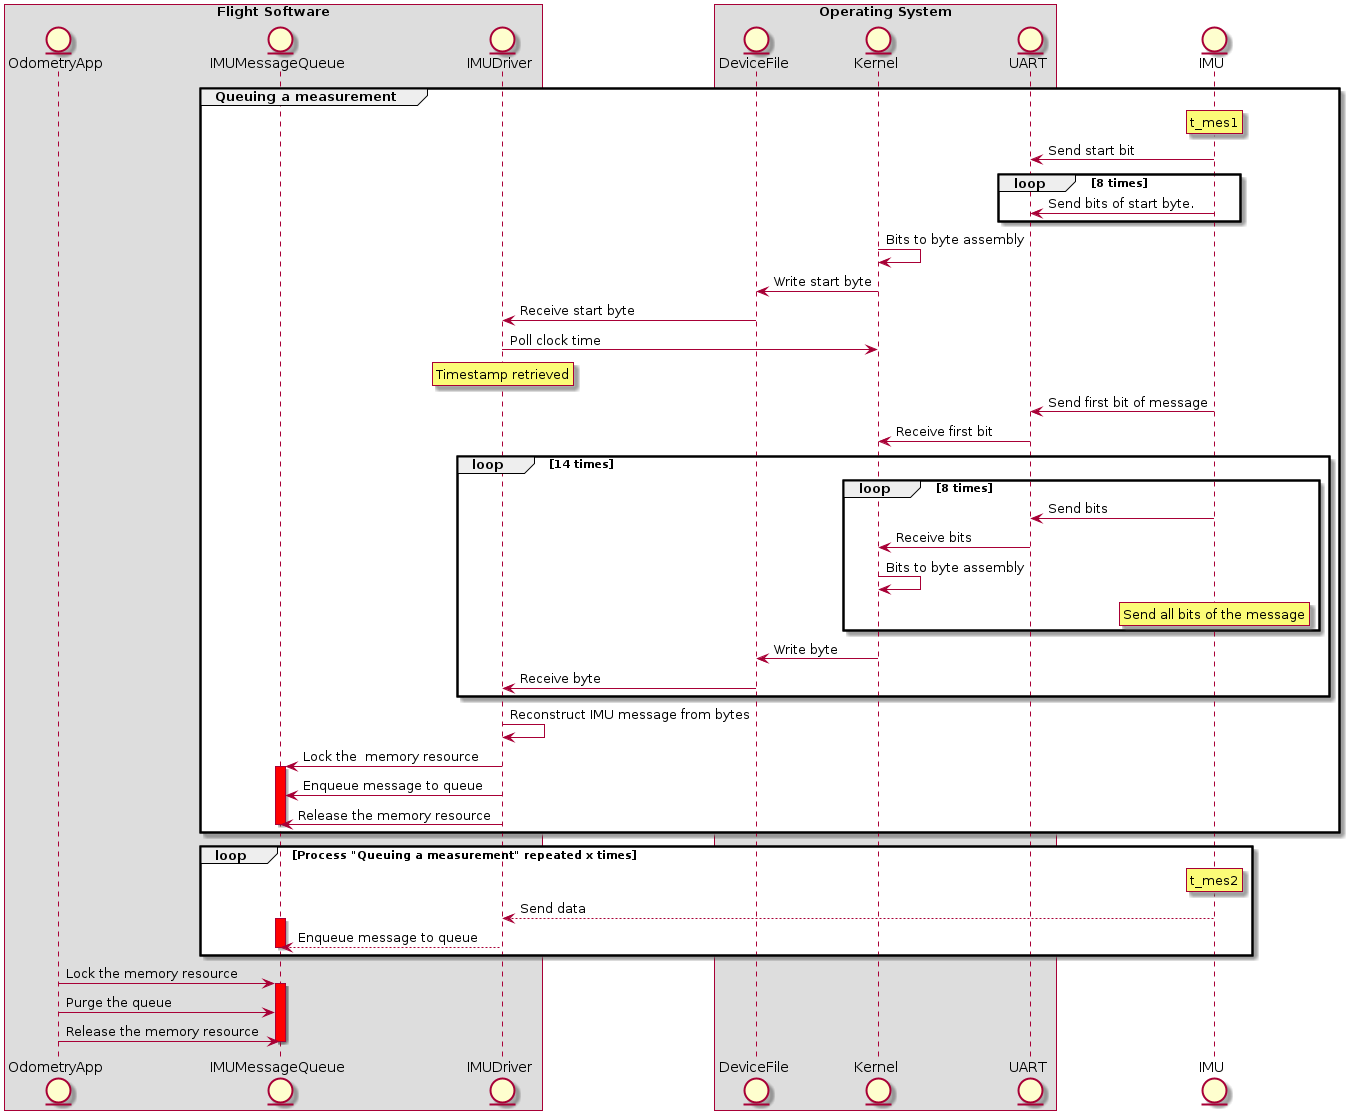
\includegraphics[width=1.0 \textwidth]{diagrams/high_level_sys_overview.png}
    \caption{High level sequence diagram of the nominal operation case}
    \label{fig-high-level-nominal}
\end{figure}

Fig.\ref{fig-high-level-nominal} describes the interaction sequence in the normal operation mode:\\
The IMU makes a new measurment at $t_{mes1}$.
It then sends a start byte to the UART to notify receiver of upcomming data frame. (See \linkreq{TS1}).
Once the first frame containing the start byte have been received, the low level UART driver of the kernel will write the byte to the device file.
Meanwhile the IMU driver is polling the kernel for the number of bytes available in the device file at high frequency. (See green line.)
As soon as one byte is availalbe, the IMU driver will read it and check if it is the start byte to detect the start of a new message (\linkreq{9}).
The IMU driver will then retrieve the clock time and use it to timestamp the measurement (\linkreq{5}).
The IMU then idle for the transfer duration of the message.
The rest of the bytes are collected by then low-level driver.
The end of the IMU driver idling time shall coincide with the last byte of the message written in device file.
The IMU driver read all the bytes and convert them to an IMU message (internal software representation).
The execution of the IMU driver shall not block the OdometryApp. Thus they must run in separate threads (\linkreq{6}).
To exchange data with the OdometryApp, the IMU driver shall store data in a shared memory queue (\linkreq{7}).\\
This process is repeated several times until the OdometryApp purge all message stored in the queue.\\
The OdometryApp will then process the IMU messages using there value and timestamp.
Therefore the driver must save timestamps together with each coresponding IMU messages (\linkreq{8}).

\subsection{Fault-tree analysis}
Because the IMU Driver is functional safety critical, it is important to derive the relevant technical safety requirements.
This section does not intend to create an exhaustive hazard and risk analysis with all possible failure modes.
This shall be done once the real hardware and usecases are known.
Instead, its intend is to create a superficial fault tree analysis to derive some of the most obvious safety relevant requirements.
We follow a top-down approach postulating a wrong trajectory reconstruction in the OdometryApp as the top event.
We categorize events as green where mitigations measures shall arguably happen outside the IMU driver and red where the IMU driver shall provide the mitigation.

\begin{figure}[H]
    \centering
    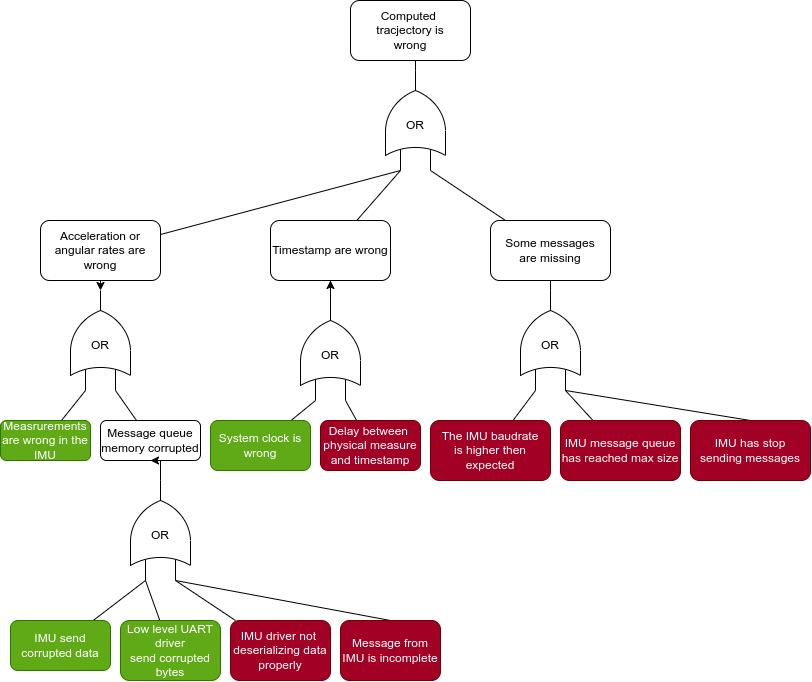
\includegraphics[width=1.0 \textwidth]{diagrams/main_fault_tree.drawio.png}
    \caption{Superficial trajectory reconstruction fault tree.}
    \label{fig-main-fault-tree}
\end{figure}

\begin{center}
\begin{tabular}{|p{5cm}|p{10cm}|}
\hline
\textbf{Failure mode} & \textbf{Mitigation} \\
\hline
IMU driver not deserializing data properly. & shall be addressed by rigorous unit testing of the implementation. \\
\hline
Message from IMU are incomplete. & shall be address by recognizing the start of a message using a start byte \linkreq{TS1}. \\
\hline
The IMU baudrate is higher than expected & in this simple example, the mitigation consist in notifying the OdometryApp when it collect the IMU messages (\linkreq{TS2},\linkreq{TS3},\linkreq{TS4}). \\
\hline
The IMU message queue has reached max size & the queue shall not grow indefinitely to prevent memory allocation issue(\linkreq(TS8)). The mitigation for the possible drop of message consist in notifying with a counter of dropped message (\linkreq{TS5},\linkreq{TS6}). \\
\hline
The IMU has stop sending messages & the mitigation consist in setting the status to NO\_DATA (\linkreq{TS3},\linkreq{TS7}). \\
\hline
Delay between physical measure and timestamp & this lag will always be present, especially with our chosen implementation of a high-level, polling driver.
To mitigate this, we implement a polling mechanism that poll at higher frequency when expecting the arrival of a start byte to mitigate the delay(\linkreq{TS9}). \\
\hline
\end{tabular}
\end{center}

\subsubsection{Definition of data frames and protocol.}
Every bytes is transmitted in a UART frame of 10 bits (1 start bit, 8 data bits, 1 stop bit).
\newline
\newline
\begin{bytefield}[bitwidth=4.1em]{10}
    \bitheader[endianness=little]{9,8,1,0}\\
    \bitbox{1}{Start bit}
    \bitbox{8}{Data bits}
    \bitbox{1}{Stop bit}
\end{bytefield}

The IMU transmit 1 start bytes and then 7 values of 2 byte eachs (14 data bytes in total).
The complete message consist if 15 frames: 1 start frame (S) and 14 data frames (D1 to D7).
\newline
\newline
\begin{bytefield}[bitwidth=2.1em]{15}
    \bitheader[endianness=little]{14,1,0}\\
    \bitbox{1}{S}
    \bitbox{14}{D1 to D7}
\end{bytefield}

This amounts to 150 bits per message.
With an output data rate of 208 Hz, the required data rate is 31200 bit/s.
We choose a typical baudrate of 38400 bit/s.
This lead to a bit transmission duration of 26 $\mu$s.
The complete message (150 bits) transmission duration is 3906 $\mu$s.
With 208 Hz, the duration between the start of two messages is 4897 $\mu$s.
This leads to an approximative 900 $\mu$s of idle time between two messages.


\subsection{Software interface definition}
We define the following structure for IMU messages.\\
To fullfill \linkreq{1}, \linkreq{8} and \linkreq{NF1},
\begin{lstlisting}[style=cppstyle]
struct ImuData {
    float a_x{};
    float a_y{};
    float a_z{};
    float omega_x{};
    float omega_y{};
    float omega_z{};
    float temperature{};
    std::chrono::nanoseconds timestamp{};
};
\end{lstlisting}
\textbf{Note:} on x86 the float type is 32 bits long which is more than the strictly necessary 16 bits. We keep float type to be compliant with the C++17 standard library.
There is no requirements on the resolution of the timestamp. This shall be derived from the actual use cases of the OdometryApp.
For the sake of higher accuracy we choose nanoseconds.
Since the measurement would come at 208 Hz only we could potentially microseconds or even miliseconds.\\

To fulfill \linkreq{TS5}.
\textbf{Note:} the queue will not fullfill \linkreq{TS8}. One could use a custom implementation later on, or this could be provided by a middelware.
\begin{lstlisting}[style=cppstyle]
struct ImuDataQueue {
  std::uint32_t dropped_message{0};
  std::queue<ImuData> data_queue{};
};
\end{lstlisting}

To fulfull \linkreq{TS2}, \linkreq{TS3}, \linkreq{TS7},
\begin{lstlisting}[style=cppstyle]
enum class ImuDriverStatus { OK, BUSY, NO_DATA };
\end{lstlisting}

\section{Use cases}
\usecase{Destkop client stays alive if device not connected}{001}{The desktop application is launched by there is no device connected. It stays on and wait until a device is connected.}

\begin{figure}[ht]
	\centering
	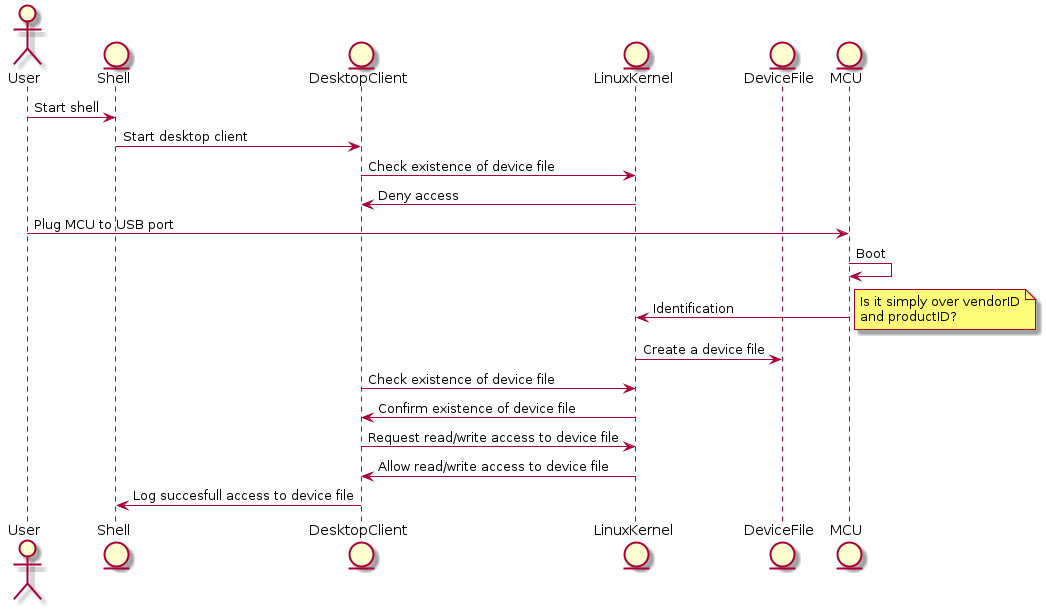
\includegraphics[width=1.0 \textwidth]{./diagrams/pc_mcu_interaction_diagram.png}
	\caption{PC-MCU interaction diagram}
	\label{fig_pc_mcu_interaction}
\end{figure}


\section{Software in the loop}
This section describe the software in the loop infrastructure and test procedure for the IMU driver. This is as follow:
\begin{itemize}
    \item The tester allocate two device files to simulate virtual serial port.
    \item The tester starts the sil application. The application immediately starts to write fake imu measurements data to the virtual device file.
    \item The tester starts the test (dummy) application that contains the driver. The driver application reads data from the virtual device file.
    \item The test application process the IMU message and determine if the test is a success or failure depending on the content.
\end{itemize}



\begin{figure}[ht]
    \centering
    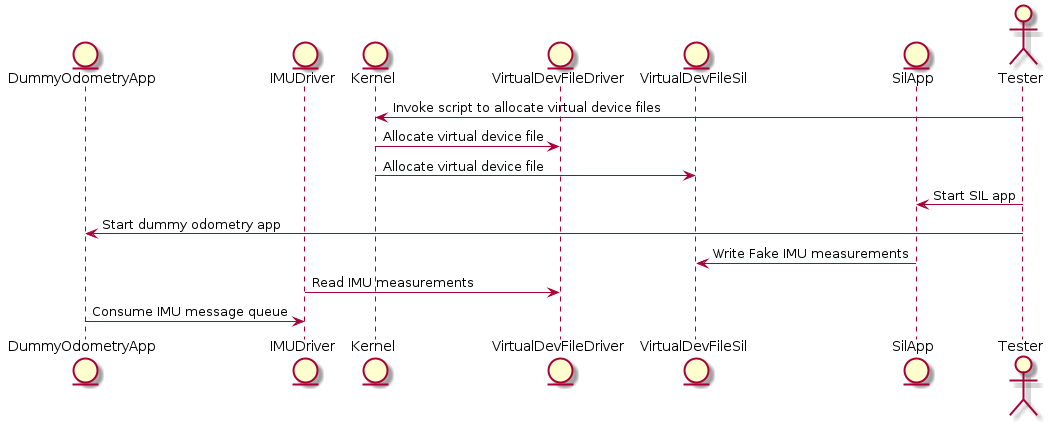
\includegraphics[width=0.75 \textwidth]{diagrams/software_in_the_loop.png}
    \caption{High level overview of SIL test procedure}
    \label{reference}
\end{figure}



\printbibliography
\end{document}
